\section{Funciones de distancia con signo (FDS)}

\SectionPage

\subsection{Primitivas sobre \(\mathbb{R}^2\)}
\begin{frame}[fragile]{Primitivas sobre \(\mathbb{R}^2\)}

    \begin{columns}
        \column{1.5in}
            \begin{figure}[H]
              \centering
              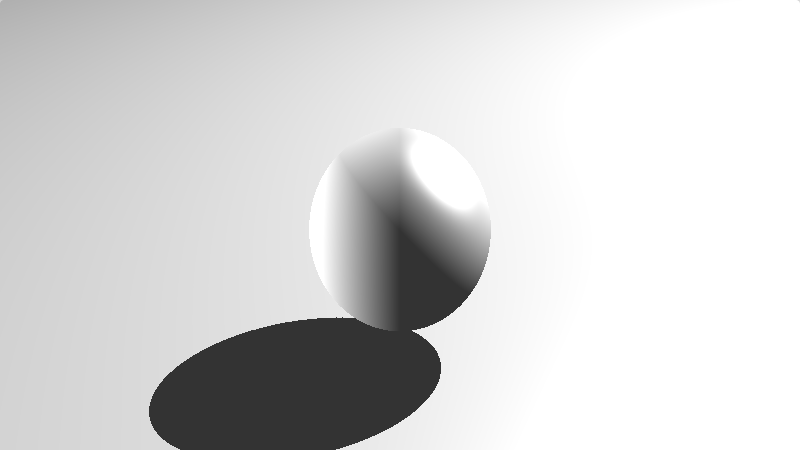
\includegraphics[width=1.0\textwidth]{imagenes/lightmodel/sombra_dura.png}
            \end{figure}
        
        \column{2.5in}
        
            \begin{lstlisting}[boxpos=t]
            float SDFCircunsferencia(vec2 p, float r){
                return length(p) - r;
            }
            \end{lstlisting}
        
    \end{columns}
    
    \begin{columns}
        \column{2.5in}
            \begin{lstlisting}
            float SDFRectangulo(vec2 p, vec2 s){
                vec2 a = abs(p) - s;
                return length(max(a, 0.0)) + min(max(a.x, a.y), 0.0);
            }
            \end{lstlisting}
    
        \column{1.5in}
            \begin{figure}[H]
              \centering
              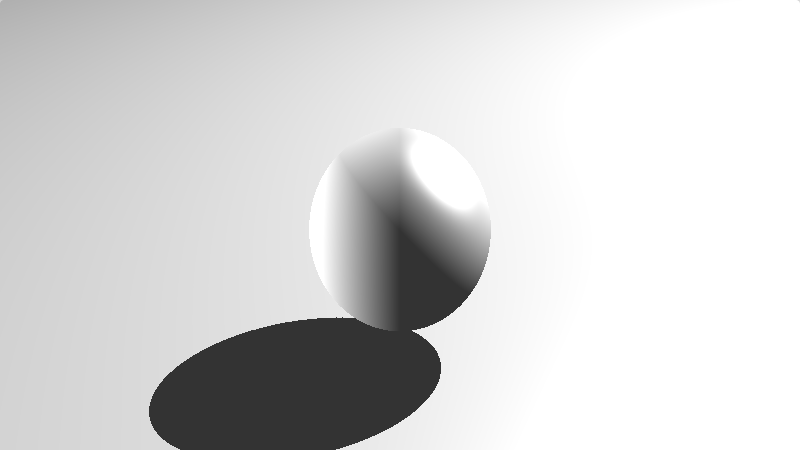
\includegraphics[width=1.0\textwidth]{imagenes/lightmodel/sombra_dura.png}
            \end{figure}
        
    \end{columns}
    
    \begin{columns}
        \column{1.5in}
            \begin{figure}[H]
              \centering
              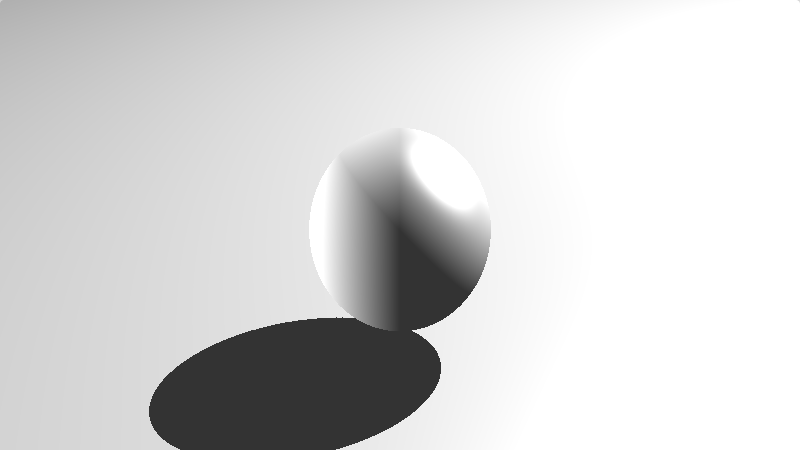
\includegraphics[width=1.0\textwidth]{imagenes/lightmodel/sombra_dura.png}
            \end{figure}
        
        \column{2.5in}
            \begin{lstlisting}
            float SDFCircunsferencia(vec2 p, float r){
                return length(p) - r;
            }
            \end{lstlisting}
        
    \end{columns}

\end{frame}

\subsection{Primitivas sobre \(\mathbb{R}^3\)}
\begin{frame}{Primitivas sobre \(\mathbb{R}^3\)}
\end{frame}